\chapter{Plasticity}


When a material deforms reversibly, its mechanical behaviour is defined as elastic. In general, there exists a particular domain of mechanical states within which the material behaves elastically. The material will deform reversibly within this domain, defined as the elastic domain and is bounded by a limit called elastic limit or yield surface \cite{simo}. Within the elastic domain, if the material is unloaded, the material will return to its original configuration. Considering only principal stresses, in 1-D case, the elastic limit is a point is known as a yield point ($\sigma_y $). In 2-D case the elastic limit is in form of  a curve and in 3-D case the elastic limit is in form of a surface. This surface is defined as yield surface\cite{borja} or loading surface\cite{simo}.
All ideas introduced in this chapter are from \cite{borja} or from \cite{simo} and form the basis on which this work has been executed.\\ 

From the yield surface the material no more remains elastic and a part of the deformation becomes non-reversible. The elastic limit mentioned above starts evolving with further strains and plasticity theories try to model this behaviour.

\begin{figure}
	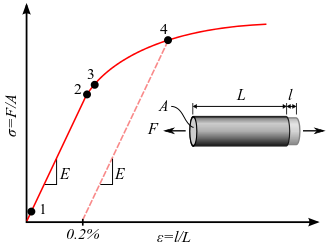
\includegraphics[width=.8\textwidth]{pics/Metal_yield.png}
	\caption{Stress–strain curve showing typical yield behavior for nonferrous alloys\cite{wiki_plas_1d}}
	\label{fig:Plas_1D}
\end{figure}

Any strain from the elastic limit is generally consist a reversible and a  non-reversible strains. Any further strain from the elastic limit are non-reversible and is called plastic strain. If the hypothesis of small strains holds true, then the total strain ($\bm  \epsilon$) in the body can be decomposed into two kind of strains. Elastic strain ($\bm \epsilon^e$) and plastic strains ($\bm \epsilon^p$). This can be expressed by the following equation:

\begin{equation}
\bm{\epsilon = \epsilon^e + \epsilon^p} \label{eq:total_strain}
\end{equation}

The stress-strain linear elastic relationship  in its broadest form is known as the generalized Hooke’s law which is given by the following equations \cite{eduardo}:
	
\begin{equation}
\bm {\sigma}=\mathbb{C}:\bm{\epsilon^e} \label{eq:hooks_law}
\end{equation}

By using the equation \ref{eq:total_strain}, we can write the equation \ref{eq:hooks_law} as,

\begin{equation}
\bm {\sigma} = \mathbb{C}:(\bm {\epsilon - \epsilon^p}) \label{eq:hooks_law_plastic}
\end{equation}

 As shown in figure \ref{fig:Plas_1D}, as the load is applied, the stress reaches the yield point at 3 and evolves to point 4. , The stress corresponding to the point 4 becoming the new elastic limit. If the load is unloaded now, the stress reduces to zero and the reversible part of the strain goes back to zero but the plastic part remains. If again loaded back, the stress now acts elastic up to the new elastic limit. This new elastic limit due to the evolution of the yield surface which over here in 1-D is a point. 
 
 \subsection*{Yield Function}
 
 
 
 To know whether the material is in the elastic domain or at the yield surface, a function called the yield function, yield criterion or loading function,(usually abbreviated as $f$) is used. Where $\bm\sigma$ is the Cauchy Stress Tensor (Simply, stress tensor) and $\bm q$ is also commonly known as Hardening Force. Yield function returns scalar value which informs of of the configuration of the mechanical state ($\bm\sigma, \bm q$) with respect to the loading surface in the material. Mathematically this is expressed as, $f:\mathbb{S} \times \mathbb{R}^m \rightarrow \mathbb{R}$ \cite{simo}
 
 \subsection*{Elastic Domain}
 We now wish to define the elastic domain,the space of plastically admissible mechanical states ($\bm\sigma, \bm q$), which is supposed to evolve when mechanical state ($\bm\sigma, \bm q$) reaches it's boundary.\cite{simo}
 
 \begin{equation}
 E_{\bm\sigma} := \left\lbrace (\bm \sigma, \bm q) \in S \times R^m | f \leq 0 \right\rbrace
 \end{equation}
 
The elastic domain corresponding to the interior of $E_\sigma$ is,
 \begin{equation}
  int (E_{\bm\sigma}) := \left\lbrace (\bm \sigma, \bm q) \in S \times R^m | f < 0 \right\rbrace
 \end{equation}
 
 and the yield surface, or loading surface, is defined as
 \begin{equation}
 \partial {E_{\bm\sigma}} =\left\lbrace (\bm \sigma, \bm q) \in S \times R^m | f = 0 \right\rbrace
 \end{equation}
 Any set of values of $(\bm\sigma, \bm q) $ that does not fall within the Elastic domain of $E_{\bm\sigma}$ are "non admissible and are ruled out in classical plasticity" \cite{simo}
 
 \subsection*{Plstic Strain and Hardening Force}
 As from the equation \ref{eq:total_strain} we see that total strain is the sum of elastic strain and plastic strain. Plastic strain is generally evolutionary, i.e., it follows generally a flow rule, expressed as following:
 
 \begin{equation}
 \dot{\bm\epsilon}^p = \dot{\lambda} \bm r(\bm \sigma, \bm q)
 \label{evol_eps_p}
 \end{equation}
 
 where $\dot{\lambda} $ is a called plastic multiplier and $\bm r$ is the flow potential.The hardening force also evolves with time and can be expressed as\cite{simo},
 
 \begin{equation}
 \dot {\bm q} = - \dot \lambda \bm H(\bm\sigma, \bm q)
 \end{equation}
% where $\dot \lambda$ is known as plastic strain rate.\cite{borja}
 
 \subsection*{Kuhn Tucker Condition}
 Consider that $E_{\bm \sigma} $ is supposed to evolve only when the stress reaches the yield surface, hence plastic strain and hardening force evolves.  There should be no evolution of  plastic strain and hardening force when the stress is not at the yield surface. Considering this, the \textit{Kuhn Tucker} complementary condition seem to be a natural conclusion, i.e., $\dot{\lambda} > 0$ only when $f(\bm \sigma, \bm q)=0$. Mathematically\cite{simo},
 
 \begin{equation}
 \dot{\lambda} \geq 0,~ f(\bm\sigma, \bm q) \leq 0\
 \end{equation}
 \textnormal{and }
 \begin{equation}
 \dot{\lambda} f(\bm\sigma, \bm q) =0
\end{equation}
\begin{equation}
 \textnormal{There also exists the consistency condition,~}
 \dot{\lambda}\dot{f}(\bm\sigma, \bm q)=0
 \end{equation}
 
 The interpretation can be simplified as\cite{simo},
 \begin{equation}
	 if,~f <0 \longleftrightarrow (\bm\sigma, \bm q) \in ~ int (E_{\sigma}=0) ~ \textnormal{(elastic)}
	 \end{equation}
	 \begin{equation}
	 if, ~f=0, ~ \longleftrightarrow (\bm\sigma, \bm q) \in ~ \partial E_{\sigma}=0, \&~
	 \dot{f}<0, ~ \dot{\lambda}=0 \textnormal{~(elastic unloading)}
	 \end{equation}
	 \begin{equation}
	 if, ~f=0, ~ \longleftrightarrow (\bm\sigma, \bm q) \in ~ \partial E_{\sigma}=0, \&~ 
	 \dot{f}=0, ~ \dot{\lambda}=0 \textnormal{~(neutral loading)}
	 \end{equation}
	 \begin{equation}
	 if, ~f=0, ~ \longleftrightarrow (\bm\sigma, \bm q) \in ~ \partial E_{\sigma}=0, \&~ 
	 \dot{f}=0, ~ \dot{\lambda}\geq 0 \textnormal{~(plastic loading)}
 \end{equation}
 
 The definition of $\bm r(\bm \sigma, \bm q)$ as defined in equation \ref{evol_eps_p} can be defined in the following ways,
 
 \begin{equation}
 	\dot{\bm \epsilon}^p = \dot{\lambda} \frac{\partial f(\bm \sigma, \bm q)}{\partial{\bm \sigma}}
 	\label{evol_eps_p_defined}
 \end{equation}
 
 In the above case, the plastic strain is directly dependent on the yield function, it is known as \textit{associative plasticity}.
 
 It might also be the case, that the plastic strain is not dependent directly on the yield function, then it is known as \textit{non-associative plasticity} and generally expressed as,
 
 \begin{equation}
 \dot {\bm \epsilon}^p = \dot{\lambda} \frac{\partial g(\bm \sigma, \bm q)}{\partial{\bm \sigma}}
 \end{equation}
 
 where $g(\bm \sigma, \bm q)$ is a function that returns a scalar and may be defined mathematically as, $g:\mathbb{S} \times \mathbb{R}^m \rightarrow \mathbb{R}$. The function is known as \textit{plastic potential}. \cite{borja}
 
 \subsection*{A Simple Introduction to Return Mapping}
 
 The evolution of yield surface is determined numerically by using an algorithm known as ``Return Mapping algorithm''\cite{simo}. It ensures the current mechanical state to remain in the space of admissible state ($E_{\bm \sigma}$).\\
 Here an algorithm for associative perfect plasticity (i.e. associative plasticity without hardening processes) is discussed following\cite{simo} and is the principal inspiration for this work.
 
 Since, plastic strain evolves with loading, the current plastic strain may be evaluated using backward euler method and can be stated as,
 
 \begin{steps}
 	\item Compute the trial stress but plugging in the total strain, to\\ $\sigma^{trial}_{n+1}=\mathbb C : (\bm \epsilon_{n+1}-\bm \epsilon_{n}^p)$
 	\item Compute the $f^{trial}_{n+1}(\bm \sigma)$ by plugging in the value of $\bm \sigma_{trial}$
 	\item If $f^{trial}_{n+1}(\bm \sigma)>0$ then go the next Step, or else go to Step 1 to compute the new total strain.
 	\item Now that $f^{trial}_{n+1}(\bm \sigma)>0$, return mapping has to be performed to set $f_{n+1}(\bm \sigma)=0$ and $\Delta \lambda$ is $>0$ A new plastic strain is calculated by preforming backward euler on the equation \ref{evol_eps_p_defined}
 	\begin{equation}
 	\bm\epsilon^p_{n+1}=\bm\epsilon^p_{n}+\Delta\lambda \frac{\partial f_{n+1}}{\partial \bm \sigma}
 	\end{equation}
 	Since Newton Iteration has to be performed, we may write,
 	\begin{equation}
 	R_{n+1}=-\bm\epsilon^p_{n+1}+\bm\epsilon^p_{n}+\Delta\lambda \frac{\partial f_{n+1}}{\partial \bm \sigma}
 	\label{eqn:Res_Eps_p}
 	\end{equation}
 	  We perform Taylor expansion on \ref{eqn:Res_Eps_p} to find the value of $\Delta \lambda$ such that.
 	\begin{equation}
 	R^{(k+1)}_{n+1}=R^{(k)}_{n+1} + \frac{\partial R^{(k)}_{n+1} }{\partial \Delta \lambda} d(\Delta \lambda)
 	\label{eq:Residual_sigma}
 	\end{equation}
 	from the equation \ref{eq:hooks_law_plastic} we can write,
 	\begin{equation}
 	\mathbb C^{-1}: \bm \sigma_{n+1}=\bm{\epsilon}_{n+1}-\bm\epsilon^p_{n+1}
 	\end{equation}
 	Using the above equation and equation \ref{eq:Residual_sigma} we can write,
 	\begin{equation}
 		R^{(k+1)}_{n+1}=R^{(k)}_{n+1} +
 		\left[\mathbb C^{-1}+\frac{\partial^2 f_{n+1}}{\partial \bm \sigma^2} \Delta\lambda\right] 
 		\frac{\partial \sigma_{n+1}}{\partial \Delta \lambda}d(\Delta \lambda)
 		+ \frac{\partial f_{n+1}}{\partial \bm \sigma}d(\Delta \lambda)
 		\label{eq:Residual_sigma_2} 
 	\end{equation}
 	Since Yield function is only dependent on $\sigma_{n+1}$, we can write, $f_{n+1}:=f(\bm \sigma_{n+1})$
 	 
 	now, considering Taylor Expansion of Yield  function, we have,
 	\begin{equation}
 		f^{k+1}_{n+1}=f^{k}_{n+1}+ \frac{\partial f^{k}_{n+1}}{\partial \bm \sigma_{n+1}} \frac{\partial \bm \sigma_{n+1}}{\partial \Delta  \lambda^k}d( \Delta  \lambda^k)
 		\label{eq:Residual_f}
 	\end{equation}
 	where $f^{k+1}_{n+1}=0$ on convergence and so does $R^{(k+1)}_{n+1}=0$ in equation \ref{eq:Residual_sigma_2}.
 	Substituting the value of $ \frac{\partial \bm \sigma_{n+1}}{\partial \Delta \lambda}d( \Delta  \lambda)$ from equation \ref{eq:Residual_sigma_2} into equation \ref{eq:Residual_f}, we get,
 	\begin{equation}
 	\left[ \mathbb{C}^{-1}+\frac{\partial^2 f_{n+1}}{\partial \bm\sigma^2_{n+1}}\Delta \lambda \right]^{-1} \left( \left[R^{(k)}_{n+1}\right] + \left[\frac{\partial f_{n+1}}{\partial \bm\sigma}\right]d(\Delta \lambda^k)\right)=f^k_{n+1}
 	\end{equation}
 	Hence,
 	\begin{equation}
 	\rightarrow d(\Delta \lambda^k) =\frac{f^k_{n+1}-\frac{\partial f_{n+1}}{\partial \sigma_{n+1}}:\left[\bm\Xi\right]:R^{(k)}_{n+1}}{\left[\frac{\partial f_{n+1}}{\partial \bm\sigma}\right]:\left[\bm\Xi\right]:\frac{\partial f_{n+1}}{\partial \bm \sigma}}
 	\end{equation}
 	where $\bm\Xi =\left[ \mathbb{C}^{-1}+\frac{\partial^2 f_{n+1}}{\partial \bm\sigma^2_{n+1}}\Delta \lambda \right]^{-1}$
 	
 	The value of $d(\Delta \lambda^k)$ is stored for the next step.
 	\item Calculate the new value of $ \frac{\partial \bm \sigma_{n+1}}{\partial \Delta \lambda}d( \Delta  \lambda)$ \
 	\begin{equation}
 	 \frac{\partial \bm \sigma_{n+1}}{\partial \Delta \lambda^k}d( \Delta  \lambda)=\bm\Xi:\left[ -R^{(k)}_{n+1}-\frac{\partial f^{k}_{n+1}}{\partial \bm \sigma_{n+1}}\right]
 	\end{equation}
 	\item Use the value of $\frac{\partial \bm \sigma_{n+1}}{\partial \Delta \lambda^k}d( \Delta  \lambda)$ to find $\Delta \epsilon^p_{n+1}$
 	\begin{equation}
 	\Delta \epsilon^{p(k)}_{n+1}=-\mathcal{C}:\frac{\partial \bm \sigma_{n+1}}{\partial \Delta \lambda}d( \Delta  \lambda)
 	\end{equation}
 	\item Next find the new values of $\epsilon^{p(k)}_{n+1}$ and $\Delta \lambda^{k}$
 	\begin{eqnarray}
 	\epsilon^{p(k+1)}_{n+1} = \epsilon^{p(k)}_{n+1}+ \Delta \epsilon^{p(k)}_{n+1}\\
 	\Delta \lambda^{k+1}=\Delta \lambda^{k}+d( \Delta  \lambda^k)
 	\end{eqnarray}
 \end{steps}

A more complex and implementation has been used in this master thesis for the return mapping algorithm. All the algorithm from the main weak forms used to the actual return mapping algorithm used, shall be discussed in the chapter ``Implementation."
 
 
 
 